\lstset{style=TigerJython,escapeinside={(*@}{@*)}}
\fboxsep=.6pt

\section{Befehle / Funktionen mit Parameter, mit \texorpdfstring{\lstinline|return|}{return}}
\subsection{Einzelne Funktionen}
\newcommand{\drawCube}[4]{
% first argument: ll position
% second argument: x shift
% 3rd argument: # of arguments
% 4th argument: size (default = 1)
% Define cube coordinates
\coordinate (A#1) at (#2,    0,     0);
\coordinate (B#1) at ({#2+#4},0,     0);
\coordinate (C#1) at ({#2+#4},#4,0);
\coordinate (D#1) at (#2,    #4,0);
\coordinate (E#1) at (#2,     0,#4);
\coordinate (F#1) at ({#2+#4}, 0,#4);
\coordinate (G#1) at ({#2+#4},#4,#4);
\coordinate (H#1) at (#2,    #4,#4);


% Draw cube
\draw[thick] (A#1) -- (B#1) -- (C#1) -- (D#1) -- cycle;
\draw[thick] (E#1) -- (F#1) -- (G#1) -- (H#1) -- cycle;
\draw[thick] (A#1) -- (E#1);
\draw[thick] (B#1) -- (F#1);
\draw[thick] (C#1) -- (G#1);
\draw[thick] (D#1) -- (H#1);
% define lower left corner of doors
% door with is defined to always be 0.2*size wide and 0.5*size high. We also define that the space between each door is the remaining width,
% i.e., if we have three doors, then the remaining space is (size-0.2*size*3)/(3+1)

% calculate how much empty space to leae between each door
\pgfmathsetmacro\emptyspace{(#4-0.2*#4*#3)/(#3+1)}

% define amount of space per door
\pgfmathsetmacro\doorsspace{0.2*#4}

\foreach \x in {1,...,#3} {	
	\pgfmathsetmacro\llCord{\emptyspace*\x+\doorsspace*(\x-1)}
	% lower door coordinate
	\coordinate (llD\x#1) at ({\llCord+#2},0,#4);
	
	% Draw doors
	\fill[blue!50, rounded corners] (llD\x#1) -- ++(0,{#4/2},0) -- ++({0.2*#4},0,0)node[pos=.5, below](in#1\x){\textcolor{blue}{\texttt{x\x}}} -- ++(0,{-#4/2},0);
	
	% lower door coordinate for value (for later annotation)
	\coordinate (llD\x#1val) at ({\llCord-.1*#4+#2},{-.2*#4},#4); % the coordinate is simple .1*size to the left of the ll corner and .2*size below.
}

% coordinate for result door
\coordinate (llDOut#1) at ({#2+#4},0,{#4*.2});
\fill[green!50, rounded corners] (llDOut#1) -- ++(0,{#4/2},0) -- ++(0,0,{#4/2})node[pos=0.8,rotate=45, below, align=center](out#1){\textcolor{black}{\tiny\texttt{out#1}\normalsize}} -- ++(0,{-#4/2},0);

% Draw a 2D rectangle around the cube
\node[fit=(E#1) (C#1), inner sep=4pt, red, dotted, draw, line width=1pt,rounded corners](dottedRect#1) {};
% annotate the two-d rect
\node[above=5pt of dottedRect#1.north west, anchor=west, align=left]{\textcolor{red}{\texttt{def a#1(\textcolor{blue}{\foreach\x in {1,...,#3}{x\x, }...})}\normalsize}};
}

Wie Sie bereits wissen, können Definitionen mit Kochrezepten verglichen werden: Sie beschreiben einen Ablauf, ohne jedoch diesen auszuführen. Damit der Ablauf ausgeführt wird, müssen Sie die Definition aufrufen. Dies kann nützlich sein, wenn sie eine Aufgabe mehrmals und in unterschiedlichen Varianten ausführen wollen, wie beispielsweise das Zeichnen einer Spirale. Eine wichtige Limitation von Definitionen war bisher, dass Sie zwar Dinge berechnen, jedoch keine Werte an das Hauptprogramm zurückgeben konnten. In diesem Kapitel lernen wir, wie Funktionen wie ``Sous-Chefs'' in einer komplexen Küche Zutaten (Parameter) entgegennehmen und Resultate an andere ``Sous-Chefs''  (Definitionen) weitergeben können.


Definitionen können zudem Inputs entgegennehmen, sogenannte \textbf{Parameter}. Wir konnten zwar bisher einen Wert einer Variable mittels \lstinline|print| drucken, Bisher konnten Sie jedoch nichts an das Hauptprogramm zurückgeben. Dies bedeutet, dass alle Variablen, die wir je in einer Definition erstellt haben, nur in dieser Definition ``lebten'' und nicht mehr zugreifbar waren, nachdem das Programm beendet wurde.

\begin{myexample}\label{ex:sum-noreturn}
Betrachten Sie folgenden Code. Weshalb führt er zu einer Fehlermeldung?
\begin{lstlisting}
def summiere(x1, x2):
    summe = x1 + x2
    
summiere(3, 5)
print(summe)
\end{lstlisting}
Die Konsole gibt folgende Meldung aus: \texttt{[Zeile: 5] NameError: name 'summe' is not defined}. Dies bedeutet, dass die Variable \lstinline|summe| auf Zeile 5 nicht existiert. Die Fehlermeldung erklärt sich dadurch, dass alle Variablen, die innerhalb einer Definition erstellt werden, nur innerhalb dieser Definition ``\textit{leben}'', also existieren. Dass Variablen mittels dem Befehl \lstinline|return| auch an das Hauptprogramm ``zurückgegeben'' werden können, lernen wir in diesem Kapitel.
\end{myexample}

Eine Funktion kann man sich vorstellen wie ein Kochrezept, das einige Zutaten entgegennimmt und ein Resultat (Gericht) zurückgibt. Die Zutaten, oder ``Inputs'', werden dabei häufig als ``\textbf{Parameter}'' bezeichnet, währenddem das fertige Gericht, oder ``Resultat'' häufig als ``\textbf{\lstinline|return|-Wert}'' bezeichnet wird. Diese Idee ist in \cref{fig:funktion-einzeln}) veranschaulicht.

\begin{figure}[H]
% Use the \drawCube macro to draw various cubes
\centering
\begin{tikzpicture}
\drawCube{1}{0}{2}{3}
\node[fill=blue!50, rounded corners] (input1) at (llD11val){3};
\node[fill=blue!50, rounded corners] (input2) at (llD21val){12};
\draw[thick,->] (input1) -- (in11);
\draw[thick,->] (input2) -- (in12);
\node[fill=green!50, rounded corners](outVal1) at (5,-.6,3){36};
\draw[thick,->] (out1) -- (outVal1);
\end{tikzpicture}
\caption{Illustration einer Funktion mit Inputs (Parametern) und Outputs (\lstinline|return|-Wert)}
\label{fig:funktion-einzeln}
\end{figure}

\begin{myexample}
Betrachten Sie nochmals den folgenden, leicht modifizierten Code aus \cref{ex:sum-noreturn}. Wenn wir den Wert mit \lstinline|return| an das Hauptprogramm zurückgeben und in einer Variable (im Hauptprogramm, auf Zeile 5) abspeichern, funktioniert der Code nun.
\begin{lstlisting}
def summiere(x1, x2):
    summe = x1 + x2
    return (*@\colorbox{CornflowerBlue}{sum\tikzmark{arrowFromEx01}me}@*)
    


(*@\colorbox{CornflowerBlue}{r\tikzmark{arrowToEx01}es}@*) = summiere(3, 5)
print(res)
\end{lstlisting}
\begin{tikzpicture}[overlay,remember picture]
   % Wert zurückgeben
	\draw[red,-stealth] (arrowFromEx01.north) to[bend left] node[align=left, pos=.3, right, fill=RoyalBlue,fill opacity=.5, text opacity=1, text=black,rounded corners] {Wert an das Hauptprogramm zurückgeben \\\textit{und} Variable speichern, z.B. \lstinline|res|} (arrowToEx01);
\end{tikzpicture}
\end{myexample}

\begin{mysubmission}
Geben seien die Höhe \texttt{h} und die Grundseite \texttt{b} eines Dreiecks. Schreiben Sie eine Funktion \lstinline|def flaeche_dreieck(h, b)|, welche den Flächeninhalt dieses Dreiecks berechnet und mit \lstinline|return| zurückgibt.

Überprüfen Sie die Korrektheit Ihrer Funktion, indem Sie sie auf Moodle hochladen.
\begin{myanswer}
\begin{lstlisting}
def flaeche_dreieck(h, b):
    return h*b/2
\end{lstlisting}
\end{myanswer}
\end{mysubmission}

\begin{mysubmission}
Geben sei eine ganze Zahl \texttt{n}. Schreiben Sie eine Funktion \lstinline|def square(n)|, welche das Quadrat von \lstinline|n| berechnet und mit \lstinline|return| zurückgibt.

Überprüfen Sie die Korrektheit Ihrer Funktion, indem Sie sie auf Moodle hochladen.
\begin{myanswer}
\begin{lstlisting}
def square(n):
    return n*n
\end{lstlisting}
\end{myanswer}
\end{mysubmission}

\begin{mysubmission}
Geben seien zwei Zahlen \lstinline|x1| und \lstinline|x2|. Schreiben Sie eine Funktion def \lstinline|maxzahl(x1, x2)|, welche die grössere der beiden Zahlen mit \lstinline|return| zurück an das Hauptprogramm gibt. Wenn beide Zahlen gleich gross sind, soll \lstinline|x2| zurückgegeben werden.

Überprüfen Sie die Korrektheit Ihrer Funktion, indem Sie sie auf Moodle hochladen.
\begin{myanswer}
\begin{lstlisting}
def maxzahl(x1, x2):
    if x1 > x2:
        return x1
    else: 
        return x2
\end{lstlisting}
\end{myanswer}
\end{mysubmission}

\begin{mysubmission}
Schreiben Sie eine Funktion, die überprüft, ob eine Liste von Zahlen sortiert ist oder nicht. Falls die Liste sortiert ist, soll die Definition den Wert \lstinline|True| zurückgeben, ansonsten den Wert \lstinline|False|.

Tipps:
\begin{enumerate}
\item Gehen Sie jedes Element der Liste mit einer Schleife durch, und überprüfen Sie, dass das Element grösser oder gleich dem vorigen Element ist.
\item \lstinline|return| bricht die Funktion ab und gibt einen Wert an das Hauptprogramm zurück. Sie können also, sobald eine Zahl in falscher Reihenfolge gefunden worden ist, direkt \lstinline|False| zurückgeben.
\item Falls Sie nie ein falsches Element gefunden haben, geben Sie am Ende der Defintion \lstinline|True| zurück.
\end{enumerate}
\begin{myanswer}
\begin{lstlisting}
def ist_sortiert(liste):
    i = 1
    while i < len(liste):
        if liste[i] < liste[i-1]:
            return False
        i += 1
    return True
\end{lstlisting}
\end{myanswer}
\end{mysubmission}
\subsection{Mehrere Funktionen}
Wozu kann so ein \lstinline|return|-Ausdruck dienen? Wenn Sie Code schreiben, wird dieser oftmals schnell komplizierter. Somit kann es hilfreich sein, die einzelnen Schritte in Unter-Programme aufzuteilen.

Zum Vergleich: stellen Sie sich vor, Sie arbeiten in einer edlen Michelin-Sterne-Küche an einem raffinierten Gericht, in das viele Arbeitsschritte involviert sind. Häufig müssen in solchen Restaurants bis zu 200 Schritte pro Gericht ausgeführt werden. Daher könnte es sinnvoll sein, einzelne Aufgaben, wie beispielsweise die Herstellung der Saucen, an Ihre Sous-Chefs zu delegieren, und eine Person zu bestimmen, die das ganze Gericht zusammenfügt. Häufig werden Funktionen genau mit solchen komplexen Aufgaben im Hinterkopf geschrieben. Diese Idee ist in \cref{fig:funktionen-mehrere} illustriert.

\begin{figure}[H]
% Use the \drawCube macro to draw various cubes
\centering
\begin{tikzpicture}
\drawCube{1}{0}{2}{3}
% feed input values into a1
\node[fill=blue!50, rounded corners] (input1) at (llD11val){3};
\node[fill=blue!50, rounded corners] (input2) at (llD21val){12};
\draw[thick,->] (input1) -- (in11);
\draw[thick,->] (input2) -- (in12);
\node[fill=green!50, rounded corners](outVal1) at (5,-.6,3){36};
\draw[thick,->] (out1) -- (outVal1);
\drawCube{2}{5.25}{3}{3}
\drawCube{3}{10.5}{2}{3}
\draw[thick,->,rounded corners] (out1) -- ++(0,-3.25,0) -- ++(3.15,0,0)node[below]{\lstinline[language=Python,style=TigerJython,basicstyle=\ttfamily]{return out1}} -- ++(4.65,0,0) -- (in31);
\end{tikzpicture}
\caption{Illustration einer Code-Struktur, bei welcher mehrere Funktionen zusammenarbeiten}
\label{fig:funktionen-mehrere}
\end{figure}

In \cref{fig:funktionen-mehrere} haben wir eine Funktion \lstinline|a1|, die zwei Parameter entgegennimmt (\lstinline|x1| und \lstinline|x2|). Mit diesen Parametern macht sie etwas (z.B. die Summe berechnen, ein Quadrat zeichnen oder irgend eine sonstige Aufgabe) und gibt danach einen neuen, berechneten Wert \lstinline|a1| zurück. Dieser kann im Hauptprogramm abgespeichert und an andere Funktionen weitergegeben werden, beispielsweise an die Funktion \lstinline|a3|.

\begin{myexample}
Stellen Sie sich vor, Sie arbeiten für einen Supermarkt und sollten den Preis Ihrer Produkte berechnen. Sie kaufen Ihre Artikel bei einem Grossverteiler ein, daher erhalten Sie auf alle Produkte 10\% Rabatt. Der Grossverteiler befindet sich im Ausland, Sie müssen also noch 7\% Mehrwertsteuer hinzufügen. Der Grossverteiler gibt Ihnen den Original-Preis Ihrer Waren \textit{vor} Rabatt und \textit{vor} Mehrwertsteuer.

Folgender Code berechnet den Endpreis, für den Sie ihre Waren verkaufen werden, indem folgende zwei Funktionen aufgerufen werden:
\begin{enumerate}
\item \lstinline|berechne_rabatt| berechnet den Preis nach Abzug eines Rabatts für ein Produkt.
\item \lstinline|berechnet_gesamtpreis| ruft \lstinline|berechne_rabatt| auf und fügt zum rabattierten Preis die Mehrwertsteuer hinzu.
\end{enumerate}

\begin{lstlisting}
def berechne_rabatt(preis, rabatt_prozent):
    rabatt = preis * (rabatt_prozent / 100)
    (*@\colorbox{CornflowerBlue}{return preis - \tikzmark{arrowFromEx11} rabatt}@*) # Gibt den Preis nach Abzug des Rabatts zurück


def berechne_gesamtpreis(preis, rabatt_prozent, mehrwertsteuer_prozent):
    (*@\colorbox{CornflowerBlue}{rabatt\tikzmark{arrowToEx11}preis}@*) = berechne_rabatt(preis, rabatt_prozent)
    mwst = rabattpreis * (mehrwertsteuer_prozent / 100)
    return (*@\colorbox{CornflowerBlue}{rabattpre\tikzmark{arrowFromEx12}is + mwst}@*)  # Gibt den Gesamtpreis inklusive Mwst. zurück


# Anwendung
preis = 100  # Basispreis in CHF
rabatt_prozent = 10  # Rabatt in %
mehrwertsteuer_prozent = 7.7  # Mehrwertsteuer in %

(*@\colorbox{CornflowerBlue}{endp\tikzmark{arrowToEx12}reis}@*) = berechne_gesamtpreis(preis, rabatt_prozent, mehrwertsteuer_prozent)
print("Der Endpreis nach Rabatt und Mehrwertsteuer ist:", endpreis)
\end{lstlisting}
\begin{tikzpicture}[overlay,remember picture]
   % Wert zurückgeben
	\draw[red,-stealth] (arrowFromEx11.north) to[bend left] node[pos=.3, right, fill=RoyalBlue,fill opacity=.5, text opacity=1, text=black,rounded corners] {Wert zurückgeben (und speichern)} (arrowToEx11);
		\draw[red,-stealth] (arrowFromEx12.north) to[bend left] node[pos=.2, right, fill=RoyalBlue, fill opacity=.5, text opacity=1, text=black,rounded corners] {Wert zurückgeben  (und speichern)} (arrowToEx12);
\end{tikzpicture}
\end{myexample}



\begin{myexample}
Mit folgendem Code können wir die Turtle eine Spirale aus mehreren Kreisen zeichnen lassen:\\
\begin{minipage}{.65\textwidth}
\begin{lstlisting}
from gturtle import *
makeTurtle()
hideTurtle()

def vieleck(umfang, ecken):
    repeat ecken:
        fd(umfang/ecken)
        rt(360/ecken)

def vieleck_muster(umfang, ecken):
    while umfang>50:
        vieleck(umfang, ecken)
        umfang-=10
        rt(10)
    
vieleck_muster(500,35)
\end{lstlisting}

\end{minipage}
\begin{minipage}{.25\textwidth}
\begin{figure}[H]
	\centering
    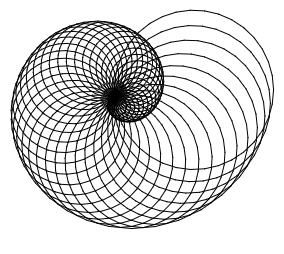
\includegraphics[keepaspectratio, width=\textwidth]{GrundlagenInfo/00_Programmieren/Figures/spirale.png}
\end{figure}
\end{minipage}\\

Leider ist unsere Turtle etwas müde und sollte nicht zu viel laufen. Daher möchten wir fortlaufend die Gesamtdistanz berechnen, um am Ende herauszufinden, ob unsere Turtle zu viel Strecke zurückgelegt hat. Dies können wir tun, indem wir die Funktion einen Wert zurückgeben lassen:
\begin{lstlisting}
from gturtle import *
makeTurtle()
hideTurtle()

def vieleck(umfang, ecken):
    repeat ecken:
        fd(umfang/ecken)
        rt(360/ecken)

def vieleck_muster(umfang, ecken):
	(*@\colorbox{CornflowerBlue}{gesamtdistanz=0}@*)
    while umfang>50:
        vieleck(umfang, ecken)
        (*@\colorbox{CornflowerBlue}{gesamtdistanz+=umfang}@*)
        umfang-=10
        rt(10)
    (*@\colorbox{CornflowerBlue}{return gesamtdistanz}@*)
    
(*@\colorbox{CornflowerBlue}{gesamtdistanz = }@*)vieleck_muster(500,35)
(*@\colorbox{CornflowerBlue}{print(gesamtdistanz)}@*)
\end{lstlisting}


\end{myexample}


Folgendes Beispiel soll dieses Prinzip konkret veranschaulichen. Stellen Sie sich vor, Sie sind SportlerIn und möchten Ihren Kalorienbedarf berechnen, um sich für auf einen kommenden Wettkampf optimal zu ernähren. Eventuell möchten Sie auch noch etwas ab- oder zunehmen, da Ihre Sportart dies erfordert. Hierzu wollen zunächst Sie Ihren täglichen Kalorienbedarf berechnen. Ihr Kalorienbedarf berechnet sich wie folgt:
\begin{enumerate}
\item Ihr Grundumsatz (englisch \gls{BMR}), d.h., ihr Grundbedarf, falls Sie sich nicht bewegen.
\item Ihr Leistungsumsatz, d.h., zusätzliche Energie, die Sie bei Aktivitäten wie Spazieren, Radfahren, Joggen usw. verbrennen.
\end{enumerate}

Beide Komponenten scheinen schwierig abzuschätzen, Sie möchten jedoch eine erste Einschätzung Ihrer \gls{BMR} haben, indem sie einige bekannte Formeln auf sich selber anwenden und diese vergleichen.

\begin{myexercise}\label{ex:bmr-simple}
Schreiben Sie eine Python-Funktion, um den Grundumsatz anhand der Harris-Benedict-Formel berechnen und geben Sie das Resultat auf der Konsole aus.
\begin{enumerate}
\item Für Männer:
\begin{align*}
\text{BMR} = & 88.362 +\\ 
& (13.397 \times \text{Gewicht in kg}) +\\ 
& (4.799 \times \text{Körpergrösse in cm}) -\\
& (5.677 \times \text{Alter in Jahren})
\end{align*}
\item Für Frauen:
\begin{align*}
\text{BMR} = & 447.593  +\\ 
& (9.247 \times \text{Gewicht in kg}) +\\ 
& (3.098 \times \text{Körpergrösse in cm}) -\\
& (4.330 \times \text{Alter in Jahren})
\end{align*}
\end{enumerate}
\begin{myanswer}
\begin{lstlisting}
def grundumsatz(gewicht, groesse, alter, geschlecht):
    """
    Berechnet den Grundumsatz (BMR) nach der Harris-Benedict-Formel.
    
    Parameter:
    - gewicht: Gewicht in kg
    - groesse: Körpergrösse in cm
    - alter: Alter in Jahren
    - geschlecht: 'mann' oder 'frau'
    
    Rückgabe:
    - BMR: Grundumsatz in Kalorien
    """
    if geschlecht == 'mann':
        bmr = 88.362 + (13.397 * gewicht) + (4.799 * groesse) - (5.677 * alter)
    elif geschlecht == 'frau':
        bmr = 447.593 + (9.247 * gewicht) + (3.098 * groesse) - (4.330 * alter)
    
    print("Der Grundumsatz beträgt:", round(bmr, 2), "Kalorien")

# Beispiel:
gewicht = 75  # kg
groesse = 180  # cm
alter = 30  # jahre
geschlecht = 'mann'

# berechne grundumsatz
grundumsatz(gewicht, groesse, alter, geschlecht)
\end{lstlisting}
\end{myanswer}
\end{myexercise}

Nun möchten wir zum Code, den Sie in \cref{ex:bmr-simple} geschrieben haben, zum Grundumsatz auch noch unsere Aktivitäten hinzufügen, allerdings können wir nun nicht mehr auf die Variable \texttt{bmr} zurückgreifen. Wie können wir das ändern? Indem wir sie an das Programm zurückgeben und speichern. Wichtige Änderungen gegebüber den Lösungs-Code aus \cref{ex:bmr-simple} sind in \colorbox{CornflowerBlue}{blau} umrandet.

\begin{minipage}{\linewidth}
\begin{lstlisting}
def grundumsatz(gewicht, groesse, alter, geschlecht):
    if geschlecht == 'mann':
        bmr = 88.362 + (13.397 * gewicht) + (4.799 * groesse) - (5.677 * alter)
    elif geschlecht == 'frau':
        bmr = 447.593 + (9.247 * gewicht) + (3.098 * groesse) - (4.330 * alter)
    
     (*@\colorbox{CornflowerBlue}{return b\tikzmark{arrowFrom}mr}@*) # gib den bmr an das Programm zurück

# Beispiel:
gewicht = 75  # kg
groesse = 180  # cm
alter = 30  # jahre
geschlecht = 'mann'

# berechne grundumsatz(*@\colorbox{CornflowerBlue}{und speichere das Resultat in einer neuen Variable resultat}@*)
(*@\colorbox{CornflowerBlue}{resu\tikzmark{arrowTo}ltat = }@*) grundumsatz(gewicht, groesse, alter, geschlecht)
(*@\colorbox{CornflowerBlue}{print("Der Grundumsatz beträgt:", round(resultat, 2), "Kalorien")}@*)
\end{lstlisting}
\end{minipage}

\begin{tikzpicture}[overlay,remember picture]
   % Wert zurückgeben
	\draw[red,-stealth] (arrowFrom.north) to[bend left] node[right, fill=RoyalBlue,text=white,rounded corners] {Wert Zurückgeben} (arrowTo);
\end{tikzpicture}

Nun haben wir eine erste Einschätzung des \gls{BMR}. Allerdings gibt es auch noch weitere Formeln, die wir gerne berechnen möchten, um einen Vergleich der verschiedenen Methoden zu erhalten.

\begin{mysubmission}\label{ex:bmr}
Schreiben Sie eine weitere Definitionen, um den \gls{BMR} anhand der Mifflin-St-Jeor-Gleichung und der Katch-McArdle-Formel zurückzugeben und berechnen Sie den Durchschnitt aller drei Formeln.
\begin{enumerate}
\item Mifflin-St-Jeor-Gleichung:
\begin{enumerate}
\item Männer: 
\begin{align*}
\text{BMR} &= 10 \times \text{Gewicht (kg)} \\
&\quad + 6.25 \times \text{Größe (cm)} \\
&\quad - 5 \times \text{Alter (Jahre)} \\
&\quad + 5
\end{align*}
\item Frauen: 
\begin{align*}
\text{BMR} &= 10 \times \text{Gewicht (kg)} \\
&\quad + 6.25 \times \text{Größe (cm)} \\
&\quad - 5 \times \text{Alter (Jahre)} \\
&\quad - 161
\end{align*}
\end{enumerate}
\item Katch-McArdle-Formel:
\begin{enumerate}
\item Grundformel:
\begin{align*}
\text{BMR} &= 370 \\
&\quad + (21.6 \times \text{FFM in kg})
\end{align*}

\item Fett-freie Masse (in kg): 
\begin{align*}
\text{FFM} &= \text{Körpergewicht (kg)} \\
&\quad \times (1 - \text{Körperfettanteil})
\end{align*}

\end{enumerate}

\end{enumerate}

\begin{myanswer}
\lstinputlisting{GrundlagenInfo/00_Programmieren/Python/bmr_functions/bmr.py}
\end{myanswer}
\end{mysubmission}

Nun haben wir eine etwas verlässlichere Einschätzung unseres Grundbedarfs. Zu diesem können wir nun auch noch die Leistungsenergie hinzufügen, um den gesamten Energiebedarf zu berechnen.

\begin{mysubmission}\label{ex:leistungsumsatz}
Berechnen Sie Ihre Leistungsenergie anhand der Tabelle \ref{tab:kcal}, indem Sie für zwei Listen erstellen: 
\begin{enumerate}
\item Eine Liste für die Zeit, während der Sie täglich einer Aktivität nachgehen
\item Eine Liste mit dem Kalorienverbrauch pro Minute für jede dieser Aktivitäten
\end{enumerate} 

\begin{table}[H]
\centering
\begin{tabular}{c|*{10}{c}}
\textbf{Gewicht (kg)} & 60 & 65 & 70 & 75 & 80 & 85 & 90 & 95 & 100 & 105 \\
\midrule\midrule
\textbf{Spazieren} & 4.5 & 5.1 & 5.4 & 5.7 & 6.0 & 6.4 & 6.7 & 7.3 & 8.0 & 9.0 \\
\midrule
\textbf{Schnelles Gehen} & 5.5 & 6.3 & 7.0 & 7.5 & 8.0 & 8.6 & 9.5 & 10.0 & 10.6 & 11.3 \\
\midrule
\textbf{Fahrradfahren} & 6.5 & 7.5 & 8.0 & 9.0 & 9.5 & 10.3 & 11.0 & 11.7 & 12.5 & 13.6 \\
\midrule
\textbf{Schwimmen} & 8.0 & 9.2 & 10.0 & 10.8 & 11.5 & 12.5 & 13.7 & 14.4 & 15.4 & 16.5 \\
\midrule
\textbf{Rudern} & 11.0 & 13.0 & 14.3 & 15.0 & 16.5 & 17.5 & 19.0 & 20.5 & 21.8 & 23.5 \\
\midrule
\textbf{Jogging} & 13.0 & 14.5 & 16.0 & 17.5 & 19.0 & 20.0 & 22.0 & 23.5 & 24.5 & 26.5 \\
\midrule
\textbf{Laufen} & 16.0 & 18.5 & 20.0 & 22.0 & 23.5 & 25.0 & 27.5 & 29.0 & 31.0 & 33.5 \\
\midrule
\textbf{Sprint} & 19.0 & 21.5 & 24.0 & 26.0 & 28.0 & 30.0 & 32.5 & 34.7 & 35.6 & 39.0 \\
\end{tabular}
\caption{Kalorienverbrauch für unterschiedliche Aktivitäten, pro Minute}
\label{tab:kcal}
\end{table}
Wenn z.B. eine 80 kg schwere Person 1 Stunde lang rudert und 20 Minuten spaziert wären die Listen wie folgt:
\begin{lstlisting}
l_zeit = [60, 20] # Zeit in Minuten
l_kcal = [16.5, 6] # Kalorien pro Aktivität
\end{lstlisting}
Schreiben Sie eine Python-Funktion \lstinline|berechne_leistungsumsatz|, um Ihren Leistungsumsatz zu berechnen. Das erwartete Resultat für das Beispiel hier wäre: \lstinline|1110| (= Summe von \lstinline|[990, 120]|). Das Resultat soll an das Hauptprogramm zurückgegeben und in einer Variable \texttt{kalorienverbrauch} gespeichert werden.
\begin{myanswer}
\lstinputlisting{GrundlagenInfo/00_Programmieren/Python/bmr_functions/leistungsumsatz.py}
\end{myanswer}

\end{mysubmission}

\begin{mysubmission}
Schreiben Sie nun eine weitere Funktion, die Ihren gesamten Energieumsatz berechnet, als Summe Ihres BMRs, den Sie in \cref{ex:bmr} berechnet haben und Ihres Leistungsumsatzes, den Sie in \cref{ex:leistungsumsatz} berechnet haben.
\end{mysubmission}

\begin{myexercise}
Schreiben Sie eine weitere Definition, die Ihren \gls{BMR} sowie alle Aktivitätsenergien summiert und zurückgibt.
\end{myexercise}

\subsection{Weitere Anwendungen}